% !TeX root = ../../main.tex
\section{Smart Device}\label{section:smart-device}

The \enquote{Smart Device} is part of the \gls{UBII} front end. It is a general-purpose client, which shares sensor data to different Topics. Because it is web-based, only hardware data which is available through the Web \gls{API} can be obtained. Since it was not designed for a specific use case, it is thought as a general-purpose or testing device. Only touch positions, touch events, orientation, and acceleration are sent to different Topics using the \gls{UBII} Client. For more specific scenarios, the smart device cannot be used, and a custom interface has to be implemented.

After implementing some improvements, the smart device client was sufficient for the experiments in this thesis. One improvement which was implemented is a full-screen mode to prevent unintentional interactions with control elements of the web browser or the \gls{OS}.
Also, a calibration system was implemented since the orientation, obtained using the Web\gls{API}, cannot be recalibrated later on~\cite{DevicesandSensorsWorkingGroup.2019}. 


\subsection{Topic Data}\label{subsection:topic-data}

The orientation is provided by the Web \gls{API} through the \lstinline{DeviceOrientation} event. It is defined by three Euler angles named \lstinline{alpha}, \lstinline{beta}, and \lstinline{gamma}, as seen in Figure~\ref{fig:webapi-device-orientation}.
While \lstinline{alpha} returns values in the range \(\left[0, 360\right)\), \lstinline{beta} only returns the range \(\left[-180, 180\right)\) and \lstinline{gamma} \(\left[-90, 90\right)\)~\cite[Chapter~4.1]{DevicesandSensorsWorkingGroup.2019}. % chktex 9
This limitation entails that no full orientation tracking is possible with this event.

\begin{figure}[H]
	\centering
	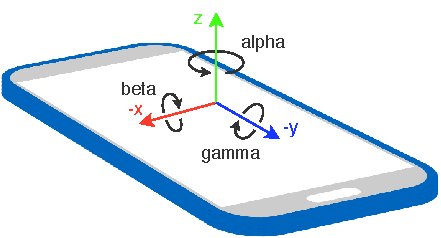
\includegraphics[height=5cm]{figures/implementation/webapi_device_orientation.pdf}
	\caption[Smart device coordinate system and orientation values]{The specification of the orientation values visualized. The \(x\) and \(y\) axes are inverted for the sake of clarity in this graphic. The arrows indicated the direction where Euler angles increases. \lstinline{alpha}, \lstinline{beta} and \lstinline{gamma} describe the three rotation angles.}\label{fig:webapi-device-orientation}
\end{figure}

% explain further role of acceleration.. only gravity is used
The Web \gls{API} also provides the \lstinline{MotionEvent} which returns multiple vectors, one being the acceleration including the gravity (\lstinline{accelerationIncludingGravity}). Since the gravity vector always points to the center of the earth, this vector can be used as a reference vector. Together with the values from the \lstinline{DeviceOrientation} event, the full orientation can be derived. The resulting orientation then has to be further processed because the acceleration vector uses the raw \gls{IMU} acceleration output, which might be very noisy.

The data from the \lstinline{DeviceOrientation} event already provides all three Euler angles as smoothed integer values. Implementing an algorithm to derive the correct orientation and further process it as the \lstinline{MotionEvent} does, would be outside the scope of this thesis. Because of this consideration, the \lstinline{DeviceOrientation} event data is used in the following experiments.

The touch position of the first finger on the smartphone display is published multiple times per second. Before sending, it is normalized to floating-point values ranging from zero to one. This keeps the data independent of the display resolution and size. Events for starting and stopping touching the screen are sent to different Topics. The acceleration of the smartphone is also sent to a Topic but is not used in any of the experiments of this thesis.


\subsection{UBII Device Definition}\label{subsection:ubii-device-definition}

The smart device is registered as a Device in the \gls{UBII} network. The Device definition in \gls{JS} can be seen in Figure~\ref{fig:ubii-device-registration}. The general structure of a Device was described in Subsection~\ref{subsection:architecture}.

\begin{figure}[H]
	\begin{lstlisting}[language=JavaScript]
    const ubiiDevice = {
      name: 'web-interface-smart-device',
      components: [{
          topic: clientId + '/web-interface-smart-device/touch_position',
          messageFormat: 'ubii.dataStructure.Vector2',
          ioType: ProtobufLibrary.ubii.devices.Component.IOType.INPUT
        },
        {
          topic: clientId + '/web-interface-smart-device/orientation',
          messageFormat: 'ubii.dataStructure.Vector3',
          ioType: ProtobufLibrary.ubii.devices.Component.IOType.INPUT
        },
        {
          topic: clientId + '/web-interface-smart-device/linear_acceleration',
          messageFormat: 'ubii.dataStructure.Vector3',
          ioType: ProtobufLibrary.ubii.devices.Component.IOType.INPUT
        },
        {
          topic: clientId + '/web-interface-smart-device/touch_events',
          messageFormat: 'ubii.dataStructure.TouchEvent',
          ioType: ProtobufLibrary.ubii.devices.Component.IOType.INPUT
        }
      ]
    };
  \end{lstlisting}
	\caption[Protobuf definition of the smart device]{The smart device's \gls{UBII} Device definition in JavaScript. It is defined by a name and a list of \gls{UBII} Components. The structure of a Device is further described in Subsection~\ref{subsection:architecture}.}\label{fig:ubii-device-registration}
\end{figure}

A Device and all Topics must be registered with a \gls{UID} for each Client because it should be possible to read the data from different devices. This allows for using multiple devices at the same time so that they can be differentiated in Interactions. If the Topic names did not include the \lstinline{clientId}, each connected device would publish to the same Topic, which would make the data unusable.

The new type \lstinline{TouchEvent} was implemented. The \gls{Protobuf} definition can be seen in Figure~\ref{fig:ubii-event-type}. It contains the two-dimensional position and the enumeration type \mbox{\lstinline{ButtonEventType}}. This type is an enumeration type which defines whether the touch interface was just touched or released.

\begin{figure}[H]
	\begin{lstlisting}[language=Protobuf]
    syntax = "proto3";
    package ubii.dataStructure;
    
    import "proto/topicData/topicDataRecord/dataStructure/vector2.proto";
    
    enum ButtonEventType {
      UP = 0;
      DOWN = 1;
    }

    message TouchEvent {
      ButtonEventType type = 1;
      ubii.dataStructure.Vector2 position = 2;
    }
  \end{lstlisting}
	\caption[Protobuf definition of the touch event]{This code shows the \gls{Protobuf} definition of the touch event (\lstinline{TouchEvent}), sent by the smart device client when users touch (\lstinline{ButtonEventType.DOWN}) or release (\lstinline{ButtonEventType.UP}) the touch screen. It is defined by a position (\lstinline{ubii.dataStructure.Vector2 position}) and whether the touch pad was touched or released (\lstinline{ButtonEventType type}).}\label{fig:ubii-event-type}
\end{figure}
